\documentclass[11pt, spanish]{memoir}
\usepackage[utf8]{inputenc}
\usepackage[spanish]{babel}
\usepackage{hyperref}
\usepackage{graphicx}
\usepackage{listings}
\usepackage{float}
\usepackage[T1]{fontenc}
\usepackage{kpfonts}
\setSingleSpace{1.1}
\SingleSpacing
\usepackage{xcolor,calc, blindtext}
\definecolor{chaptercolor}{gray}{0.8}
% helper macros
\newcommand\numlifter[1]{\raisebox{-2cm}[0pt][0pt]{\smash{#1}}}
\newcommand\numindent{\kern37pt}
\newlength\chaptertitleboxheight
\makechapterstyle{hansen}{
  \renewcommand\printchaptername{\raggedleft}
  \renewcommand\printchapternum{%
    \begingroup%
    \leavevmode%
    \chapnumfont%
    \strut%
    \numlifter{\thechapter}%
    \numindent%
\endgroup%
}
  \renewcommand*{\printchapternonum}{%
    \vphantom{\begingroup%
      \leavevmode%
      \chapnumfont%
      \numlifter{\vphantom{9}}%
      \numindent%
      \endgroup}
    \afterchapternum}
  \setlength\midchapskip{0pt}
  \setlength\beforechapskip{0.5\baselineskip}
  \setlength{\afterchapskip}{3\baselineskip}
  \renewcommand\chapnumfont{%
    \fontsize{4cm}{0cm}%
    \bfseries%
    \sffamily%
    \color{chaptercolor}%
  }
  \renewcommand\chaptitlefont{%
    \normalfont%
    \huge%
    \bfseries%
    \raggedleft%
  }%
  \settototalheight\chaptertitleboxheight{%
    \parbox{\textwidth}{\chaptitlefont \strut bg\\bg\strut}}
  \renewcommand\printchaptertitle[1]{%
    \parbox[t][\chaptertitleboxheight][t]{\textwidth}{%
      %\microtypesetup{protrusion=false}% add this if you use microtype
      \chaptitlefont\strut ##1\strut}%
}}
\chapterstyle{hansen}
\aliaspagestyle{chapter}{empty} % just to save some space
\begin{document}
\chapter{Instalación de MADMex}
Para instalar el sistema MADMex, es necesario contar con una instalación de GDAL funcionando correctamente. También es necesario contar con un interprete de Python y que el mismo se encuentre instalado en las variables de entorno, de modo que sea ejecutable desde una consola de comandos.

Para lograr esto, descargamos el instalador de python desde:

\url{https://www.python.org/ftp/python/2.7/python-2.7.amd64.msi}

ejecutando el instalador y siguiendo las configuraciones por defecto, python quedará instalado en la dirección:


\begin{lstlisting} 
C:\Python27
\end{lstlisting}

Para que python sea visible desde cualquier carpeta en la consola de comandos, es necesario ejectutar la siguiente instrucción:

\begin{lstlisting} 
SET PATH=%PATH%;C:\Python27
\end{lstlisting}

\begin{figure}[H]
\centering
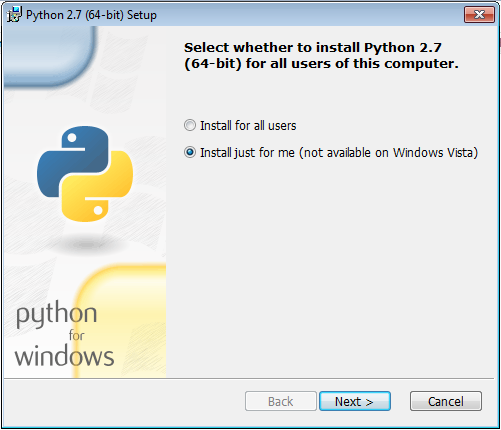
\includegraphics[width=14cm]{python2.png}
\end{figure}

\begin{figure}[H]
\centering
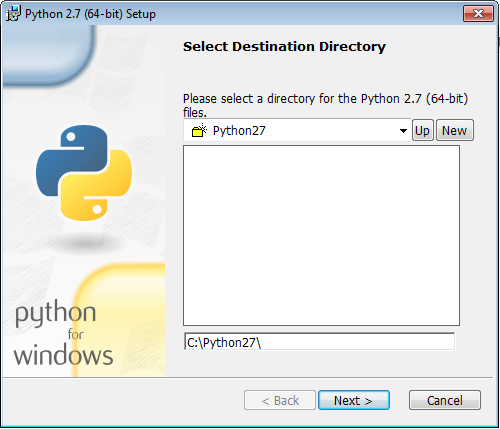
\includegraphics[width=14cm]{python3.png}
\end{figure}

\begin{figure}[H]
\centering
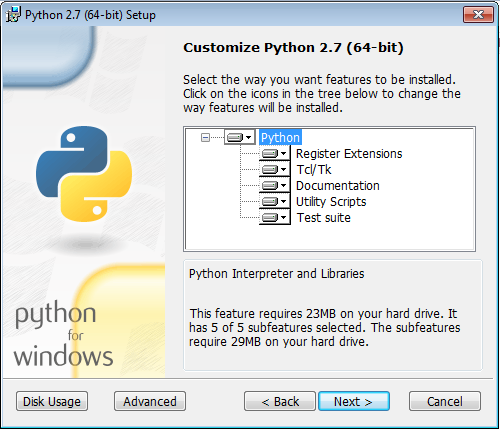
\includegraphics[width=14cm]{python4.png}
\end{figure}

\begin{figure}[H]
\centering
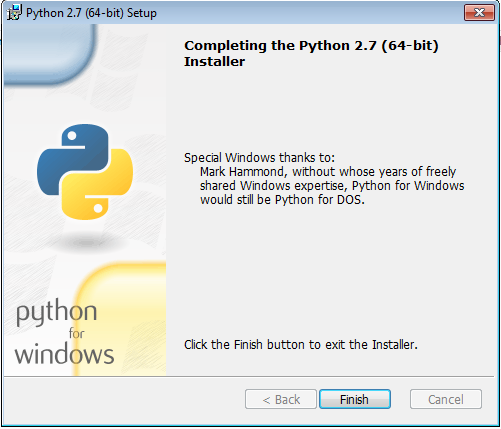
\includegraphics[width=14cm]{python5.png}
\end{figure}

Madmex tiene ciertas dependencias externas, en el caso del preprocesamiento de imágenes,
es necesario contar con geoalchemy2 y con numpy. Para instalarlos, una herramienta que resulta muy útil es pip. Para instalar pip se descarga el siguiente script:

\url{https://bootstrap.pypa.io/get-pip.py}

una vez descargado, se navega hasta la ubicación del mismo (usualmente en la carpeta de Descargas) y se ejecuta:

\begin{lstlisting} 
python get-pip.py
\end{lstlisting}

\begin{figure}[H]
\centering
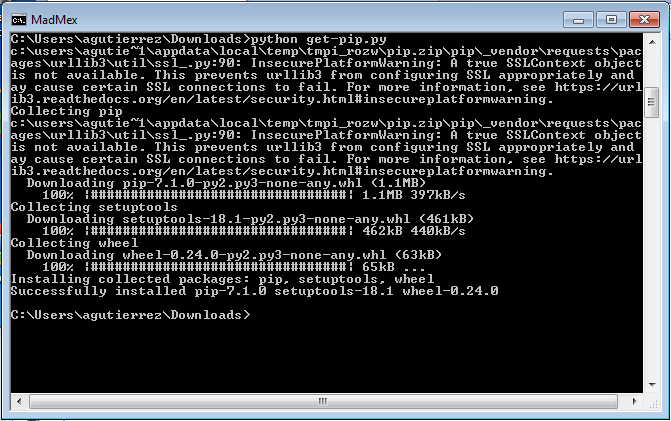
\includegraphics[width=14cm]{pip.png}
\end{figure}

para verificar que la herramienta se instaló correctamente se puede ejecutar el siguiente comando:

\begin{lstlisting} 
python -m pip install -U pip
\end{lstlisting}

este comando intenta actualizar la herramienta, en caso de que la instalación haya sido realizada correctamente, aparecerá un mensaje de que la herramienta se encuentra al dia. Esta herramienta sirve para facilitar la instalación de nuevos paquetes en nuestro intérprete de python. Para insalar el primer requisito, usamos la siguiente instrucción (el directiorio no importa ya que python ya ha sido agregado al path)

\begin{lstlisting} 
python -m pip install geoalchemy2==0.2.5
\end{lstlisting}

\begin{figure}[H]
\centering
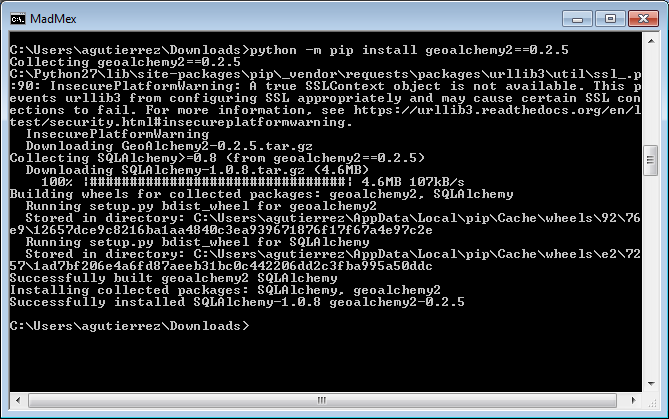
\includegraphics[width=14cm]{geoalchemy.png}
\end{figure}

Para instalar numpy, un paso extra es necesario. Numpy requiere de un compilador de C++ que es distribuido gratuitamente por Microsoft. Para instalar dicho requisito es necesario descargar el ejecutable desde:

\url{http://aka.ms/vcpython27}

Una vez instalado, procedemos a instalar numpy de la siguiente forma:

\begin{lstlisting} 
python -m pip install numpy==1.9.2
\end{lstlisting}

\begin{figure}[H]
\centering
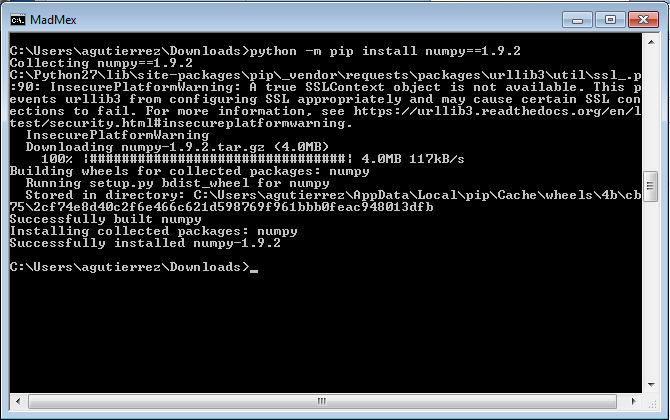
\includegraphics[width=14cm]{numpy.png}
\end{figure}

Por último es necesario instalar el módulo de gdal y los bindings necesarios para poder usar dicho modulo desde python. Para instalar GDAL obtenemos el instalador en:

\url{http://download.gisinternals.com/sdk/downloads/release-1500-x64-gdal-1-11-1-mapserver-6-4-1/gdal-111-1500-x64-core.msi}

ejecutandolo y dejando las configuraciones por defecto, se instalará en la carpeta:

\begin{lstlisting} 
C:\Program Files\GDAL
\end{lstlisting}

\begin{figure}[H]
\centering
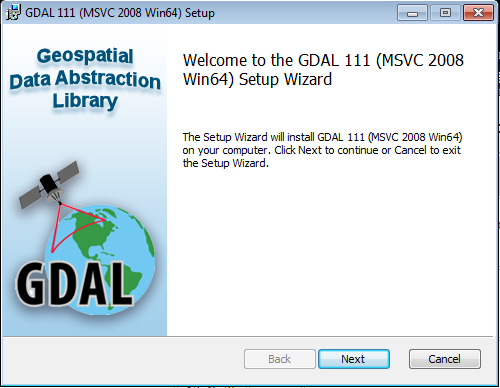
\includegraphics[width=14cm]{gdal1.png}
\end{figure}

\begin{figure}[H]
\centering
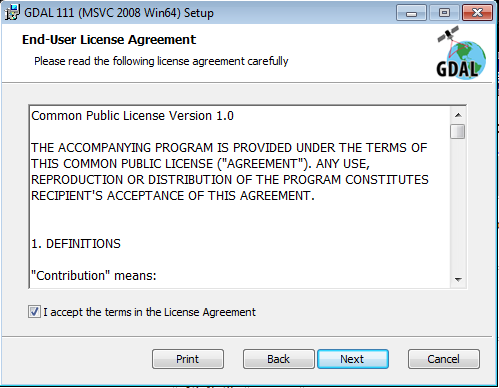
\includegraphics[width=14cm]{gdal2.png}
\end{figure}

\begin{figure}[H]
\centering
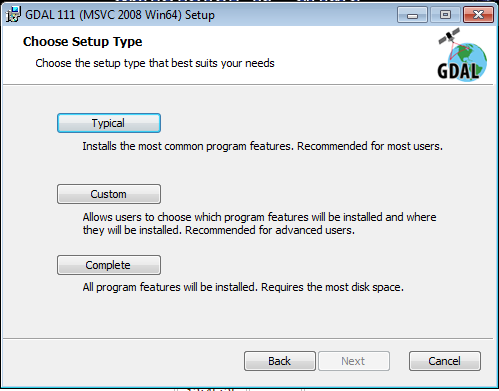
\includegraphics[width=14cm]{gdal3.png}
\end{figure}

\begin{figure}[H]
\centering
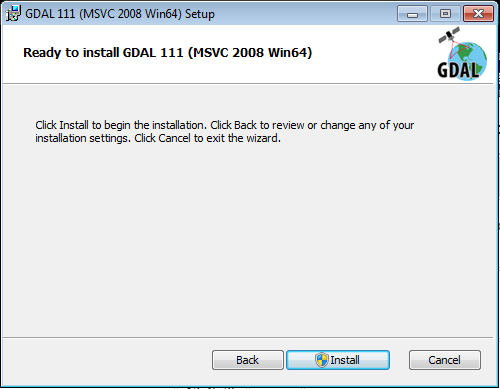
\includegraphics[width=14cm]{gdal4.png}
\end{figure}

\begin{figure}[H]
\centering
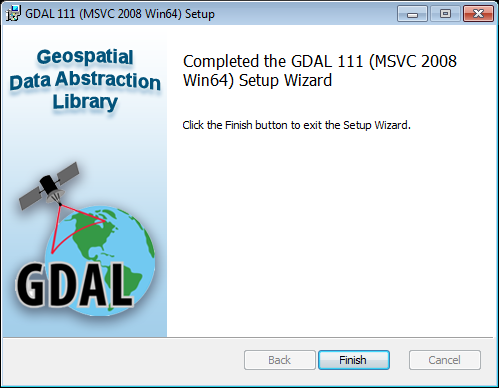
\includegraphics[width=14cm]{gdal5.png}
\end{figure}

en el caso de los bindings, se instalan de la misma manera, descargando el instalador desde:

\url{http://download.gisinternals.com/sdk/downloads/release-1500-x64-gdal-1-11-1-mapserver-6-4-1/GDAL-1.11.1.win-amd64-py2.7.msi}

el instalador encontrará la dirección del python instalada usando de registro de Windows, por lo que no será necesario configurar nada manualmente.

\begin{figure}[H]
\centering
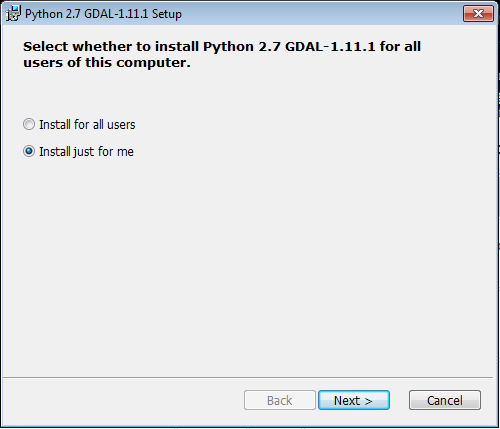
\includegraphics[width=14cm]{bindings1.png}
\end{figure}

\begin{figure}[H]
\centering
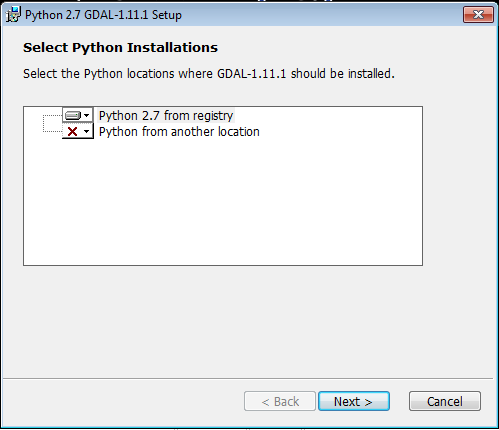
\includegraphics[width=14cm]{bindings2.png}
\end{figure}

\begin{figure}[H]
\centering
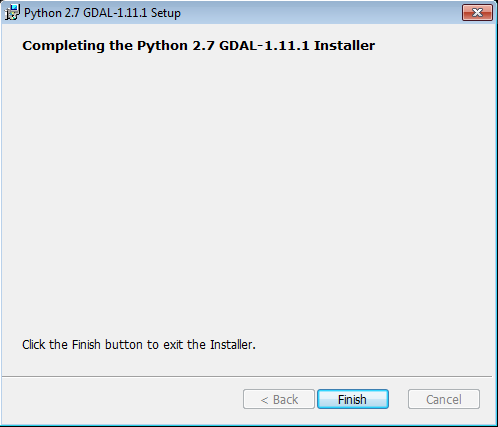
\includegraphics[width=14cm]{bindings3.png}
\end{figure}

Una vez que estos pasos han sido completados es necesario agregar nuestras instalaciones al path de Windows. El path de Windows es el conjunto de directiorios visibles para la consola de comandos desde cualquier dirección. Para poder ejecutar python desde cualquier sitio, es necesario agregar:

\begin{lstlisting} 
C:\Python27
\end{lstlisting}

a la lista de directiorios. Lo mismo ocurre con GDAL y otras carpetas con herramientas útiles. Para configurar una consola de comandos con estas características es necesario crear un acceso directo al ejecutable de la consola, que se encuentra en la dirección:

\begin{lstlisting} 
C:\Windows\System32
\end{lstlisting}

bajo el nombre:

\begin{lstlisting} 
cmd.exe
\end{lstlisting}

haciendo click derecho, elegimos la opción "Crear acceso directo" y creamos el acceso directo donde queramos, por ejemplo, en el escritorio: 

\begin{figure}[H]
\centering
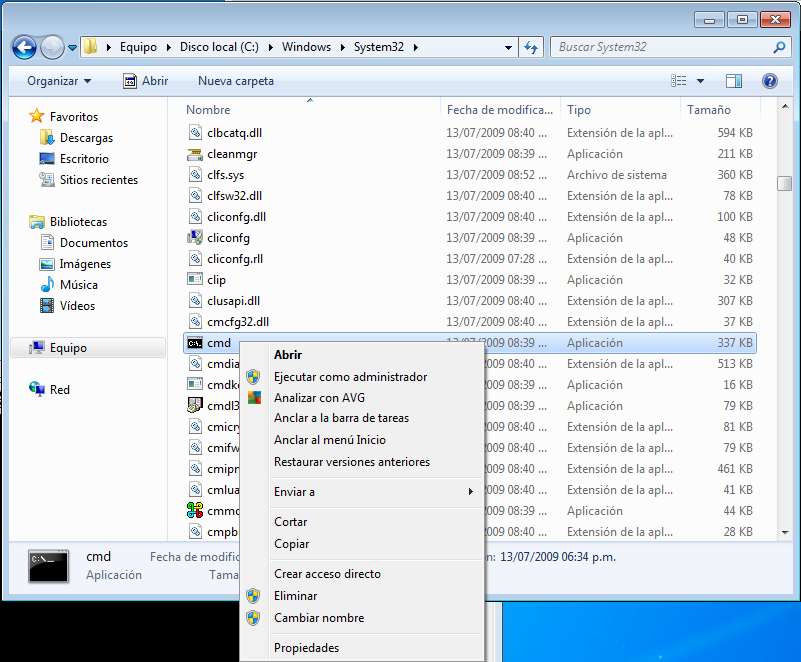
\includegraphics[width=14cm]{acceso_directo1.png}
\end{figure}

Usando notepad, creamos un archivo de texto con el siguiente contenido:

\begin{lstlisting} 
@SET PATH=%PATH%;C:\Python27;C:\Program Files\GDAL
@SET GDAL_DATA=C:\Program Files\GDAL\gdal-data
@SET GDAL_Driver_PATH=C:\Program Files\GDAL\gdalplugins
@SET PYTHONPATH=%PYTHONPATH%;C:\Python27\Lib
\end{lstlisting}

\begin{figure}[H]
\centering
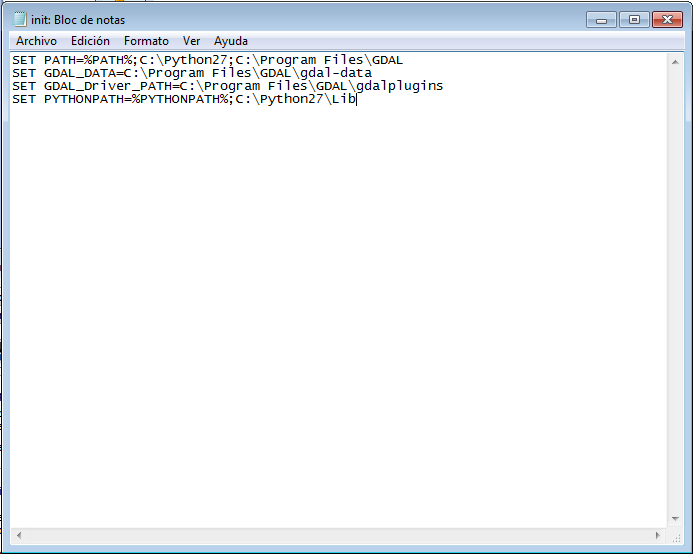
\includegraphics[width=14cm]{acceso_directo2.png}
\end{figure}

elegimos la opción "Guardar como" y en "Tipo" la opción "Todos los archivos" nombramos el archivo como init.bat y cerramos notepad. 

\begin{figure}[H]
\centering
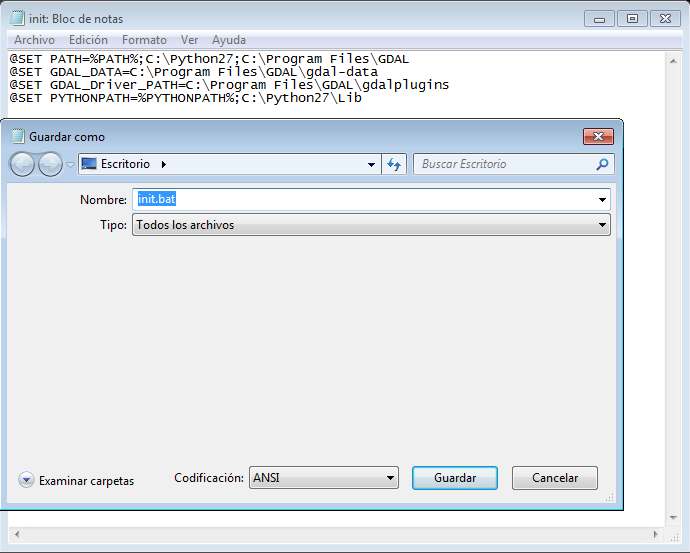
\includegraphics[width=14cm]{acceso_directo3.png}
\end{figure}

Lo que haremos con este archivo de instrucciones es decirle a Windows que cada vez que iniciemos la terminal a través de nuestro acceso directo, ejecute estas instrucciones, de este modo no tendremos que hacerlo manualmente cada vez. Para configurar este comportamiento en el menú, que aparece al presionar el boton derecho del mouse sobre el ícono de nuestro acceso directo, elegimos "Propiedades". En la ventana de propiedades, dentro de la pestaña "Acceso directo" ponemos en "Destino" el siguiente comando:

\begin{lstlisting} 
C:\Windows\System32\cmd.exe /k "%USERPROFILE%\Desktop\init.bat"
\end{lstlisting}

en este caso, debido a que creamos el init.bat en el escritorio, en otro caso se tendría que dar la dirección de dicho archivo. En el campo "Iniciar en" podemos poner la dirección en la cual deseamos que la consola sea abierta, en mi caso uso la dirección por default del usuario.

\begin{lstlisting} 
%USERPROFILE%
\end{lstlisting}

Una vez que todos los prerequisitos han sido instalados, podemos probar si nuestro ambiente de pyhton está configurado correctamente, iniciando una consola de python y probando los siguientes comandos:

\begin{lstlisting}
import gdal
import numpy
import geoalchemy2
\end{lstlisting}

en caso de que todos los pasos hayan resultado exitosos, ninguno de estos comandos producirá un error y significa que nuestro ambiente está listo para instalar madmex.

Se accede a la página localizada en:

\url{http://nodo2.conabio.gob.mx:8080/job/Madmex/}

\begin{figure}[H]
\centering
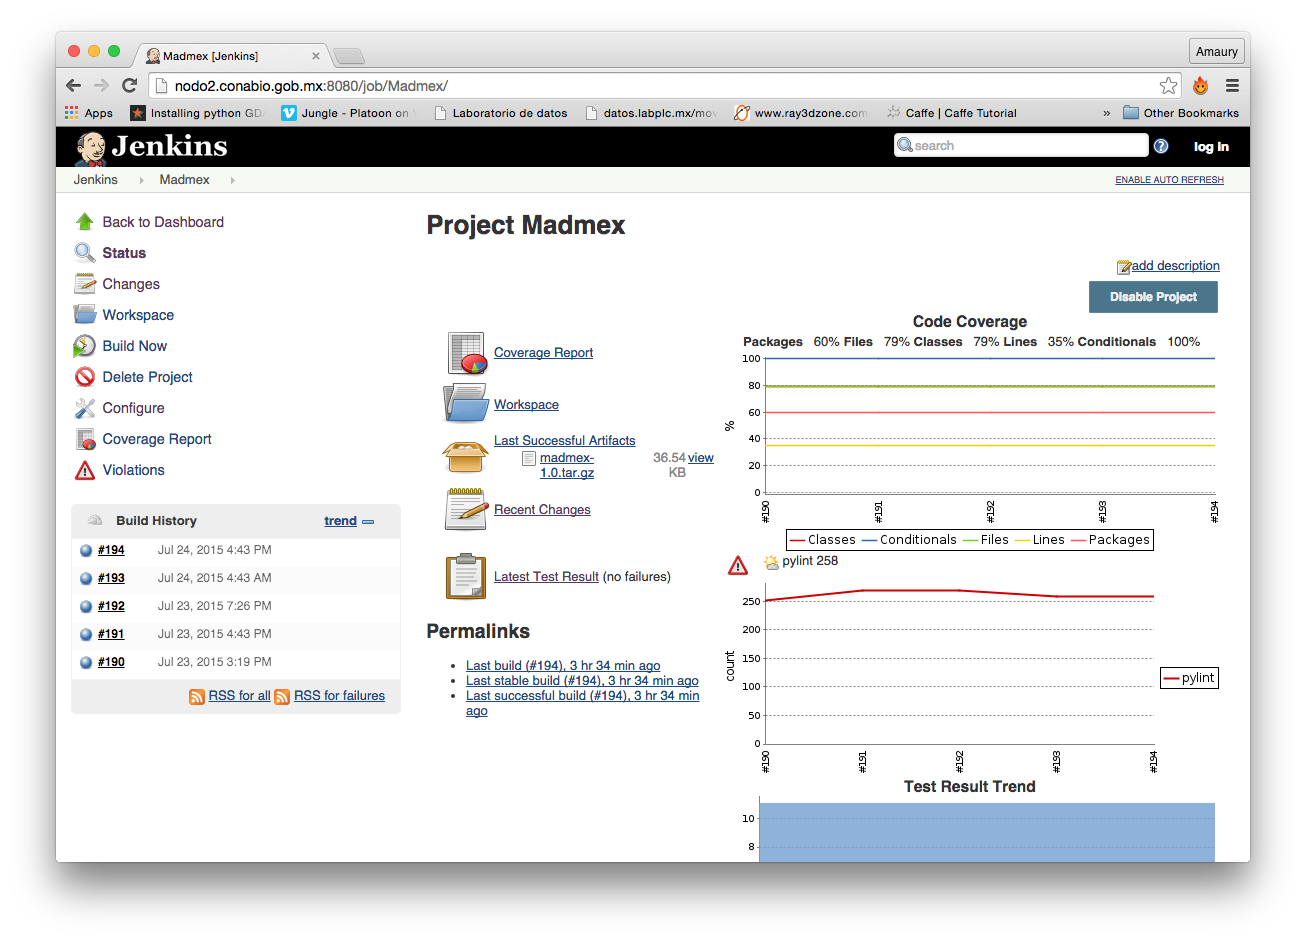
\includegraphics[width=14cm]{screen1.png}
\caption{Pantalla de descarga. \label{overflow}}
\end{figure}
Al hacer click en el link madmex-1.0.tar.gz se descargará un paquete que incluye
los archivos necesarios para instalar el sistema. Una vez que se cuenta con el
archivo tar, es necesario descomprimirlo (Un descompresor de archivos zip puede
hacerlo, uno open source se puede encontrar en \url{http://www.7-zip.org/}). La
instalación se realiza desde la consola. Para abrir la consola de comandos se puede
escribir cmd en el buscador del Inicio.

\begin{figure}[H]
\centering
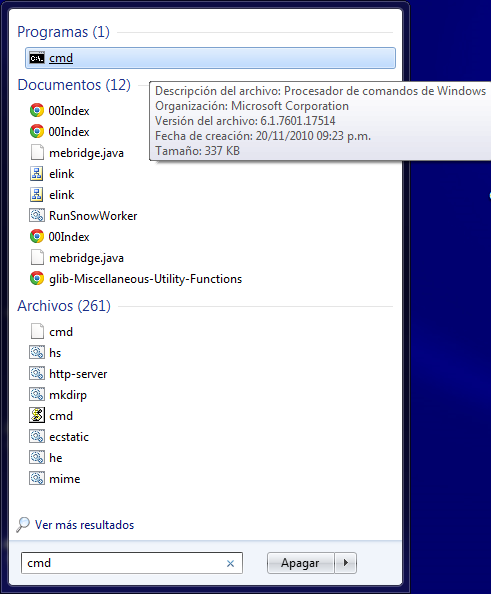
\includegraphics[width=6cm]{command1.png}
\caption{Pantalla de descarga. \label{overflow}}
\end{figure}

Navegando hasta la carpeta descomprimida
se introduce el siguiente comando:

\begin{figure}[H]
\centering
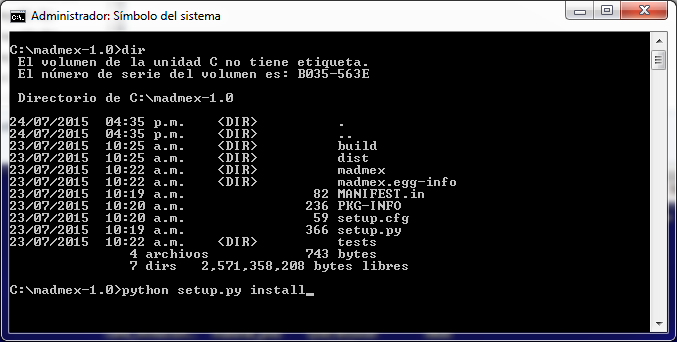
\includegraphics[width=14cm]{command2.png}
\caption{Pantalla de descarga. \label{overflow}}
\end{figure}
En caso de que el comando anterior funcione correctamente, la salida del sistema sera
 algo como:
\begin{figure}[H]
\centering
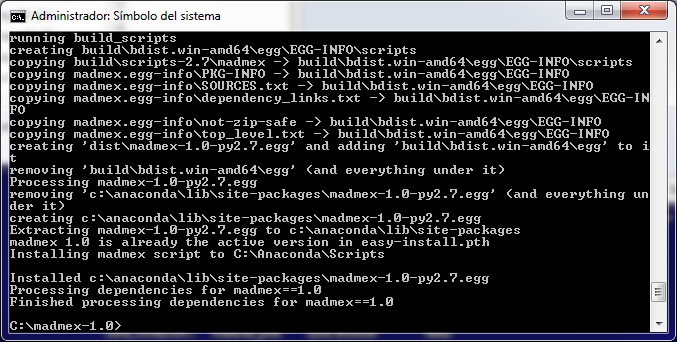
\includegraphics[width=14cm]{command3.png}
\caption{Pantalla de descarga. \label{overflow}}
\end{figure}

Por último para realizar el preprocesamiento de las imágenes se escribe el comando:

\begin{figure}[H]
\centering
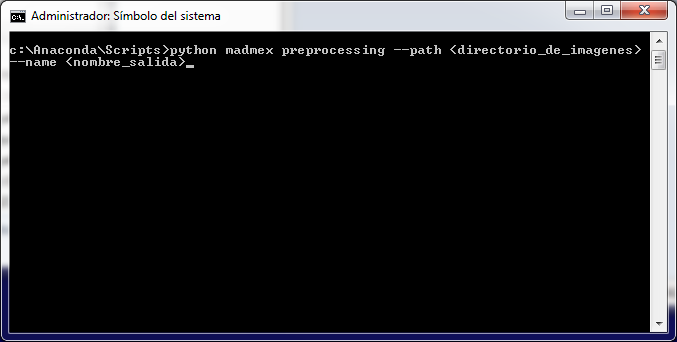
\includegraphics[width=14cm]{command4.png}
\caption{Pantalla de descarga. \label{overflow}}
\end{figure}


\end{document}
